\documentclass[a4paper,spanish]{article}
\usepackage[spanish]{babel}
\usepackage[ansinew]{inputenc}
\usepackage[T1]{fontenc}
\usepackage{graphicx}
\usepackage{multicol}
\usepackage{longtable}
\usepackage{array}
\usepackage{multirow}

\renewcommand{\tablename}{Tabla}
\renewcommand{\S}{Excepciones, colecciones y polimorfismo}
\author{Examen tercera evaluaci�n}
\title{\textbf{\S}}
\date{\today}

\begin{document}
\maketitle 
%\tableofcontents
%\newpage
\vspace{2cm}
\begin{center}
\begin{large}
\textbf{Diagrama UML de la aplicaci�n}
\end{large}
\end{center}\par 
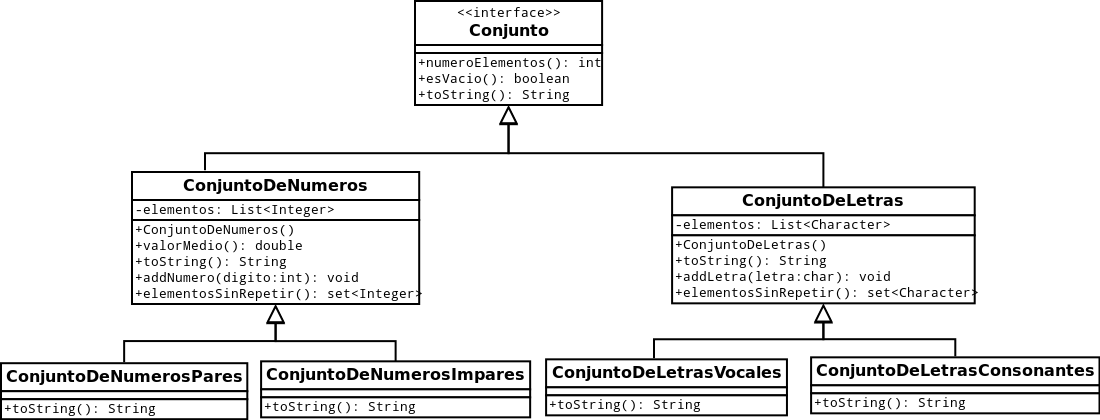
\includegraphics[scale=0.35]{UML1.png}
\vspace{0.5cm}
\section*{Ejercicio 1}
Crea un proyecto denominado \emph{ejercicio1} y en �l incorpora las correspondientes clases, teniendo en cuenta las caracter�sticas que se te indican a contiunuaci�n.
\begin{itemize}
\item Crea las clases que se te piden en el diagrama UML anterior.
\item En la \emph{interface} el metodo \emph{numeroElementos} devuelve el n�mero total de elementos que tiene ese conjunto. El m�todo \emph{esVacio} nos dice \emph{true} si no contiene ning�n elemento. El m�todo \emph{toString} imprime los valores del conjunto.
\item Los constructores de las clases \emph{ConjuntoDeNumeros} y \emph{ConjuntoDeLetras} inicializan las correspondientes listas a listas vac�as.
\item El m�todo \emph{toString} en las clase anteriores debe devolver el literal \emph{son n�meros} para el caso de la clase \emph{ConjuntoDeNumeros} y  \emph{son letras} para el caso de la clase \emph{ConjuntoDeLetras}. Para las clases \emph{ConjuntoDeNumeroPares}, \emph{ConjuntoDeNumeroImpares}, \emph{ConjuntoDeLetrasVocales} y \emph{ConjuntoDeLetrasConsonantes} debe devolver \emph{son pares}, \emph{son impares}, \emph{son vocales} y \emph{son consonantes}, respectivamente para los m�todos \emph{toString}. En todos estos m�todos se debe incorporar el valor del \emph{toString} de la interface.
\item El m�todo \emph{valorMedio} devuelve el valor medio de los elementos del conjunto.
\item Los m�todo \emph{addNumero} y \emph{addLetra} a�ade un elemento a cada listas correspondiente.
\item El m�todo \emph{elementosSinRepetir}, devuelve un \emph{Set} con los elementos sin repetir de los correspondientes conjuntos.
\item Crea una clase denominada \emph{TestConjuntos} con un m�todo main que cree cuatro objetos de tipo \emph{ConjuntoDeNumeroPares}, \emph{ConjuntoDeNumeroImpares}, \emph{ConjuntoDeLetrasVocales} y \emph{ConjuntoDeLetrasConsonantes}, pero el tipo declarado debe ser \emph{Conjunto}.
\item En dicha clase se lee los datos mediante la clase \emph{Scanner} desde el fichero \emph{numeros.txt} para el caso de los n�meros. Y mediante otro \emph{Scanner} lee los datos de letras del fichero \emph{letras.txt}
\item Una vez le�do recorre las colecciones correspondientes y nos diga los datos de acuerdo al m�todo \emph{toString} de cada objeto.
\item Despu�s de recorrer dichas colecciones debemos saber si cada conjunto est� vac�o o no.
\item Tambi�n nos diga el n�mero de elementos de cada elementos
\item Adem�s el n�mero de elementos sin repetir de cada objeto.
\item Por �ltimo imprime los datos ordenados de dichas listas.
\item Crea un un objeto de la clase \emph{Map} para que guarde los diez primeros valores de las listas sin repetir en dicho objeto, de manera que cada registro est� formado por una clave que sea la letra y como valor el n�mero.
\item Crea dentro de esta clase \emph{TestConjuntos} los siguientes m�todos est�ticos siguientes:
\begin{itemize}
\item \emph{imprimirHash} que reciba como par�metro al objeto anterior e imprima los datos del \emph{Hash} tanto la clave como el valor.
\item \emph{imprimirValoresDelHash} que reciba como par�metro un objeto de tipo Integer y nos diga el valor de dicha clave, en el caso que exista.
\item \emph{devolverClaves} que reciba al objeto anterior y devuelva un \emph{Set} con los datos de las claves.
\item Comprueba el funcionamiento de dichos metodos estaticos.

\end{itemize}
\end{itemize}
\section*{Cuestion}
En un fichero de texto contesta a las siguientes dos cuestiones:
\begin{itemize}
\item �Qu� hubiera ocurrido si no se sobrescriben el m�todo \emph{toString} en todas las clases?
\item �Que hubiera ocurrido si no se declaran los objetos como \emph{Conjunto}?
\end{itemize}
\section*{Criterios de evaluacion}
Los criterios de evaluaci�n son los indicados a continuaci�n:\par 
\vspace*{0.5cm}
\begin{tabular}{|c|c|}
\hline
\textbf{CRITERIO EVALUACION} & \textbf{PUNTUACION} \\
\hline
Archivo Conjunto.java bien & 0.5 ptos.\\
\hline
Archivos java de las clases hijas inferiores & 0.5 ptos\\
\hline
Archivo ConjuntoDeNumeros.java bien & 1 pto. \\
\hline
Archivo ConjuntoDeLetras.java bien & 1 pto.\\
\hline
Lectura de los datos con Scanner en TestConjuntos1 correctos & 2 ptos.\\
\hline 
Impresi�n de datos correctos en TestConjuntos & 2 ptos.\\
\hline
Creaci�n del Map y m�todos asociados bien & 2 ptos.\\
\hline
Imprimir los datos de las listas ordenados & 1 pto.\\
\hline
Cuestiones correctas & 1 pto\\
\hline
\end{tabular}
\section*{Subida de ficheros}
Comprime el directorio de trabajo de eclipse y comprimelo junto al fichero de las cuestiones y lo subes a la plataforma.
\end{document}
